\documentclass[12pt]{article}
\usepackage{lingmacros}
\usepackage{tree-dvips}
\usepackage{graphicx}
\begin{document}

\section{Heap Buffer overflow}

\subsection{Protection}
\begin{itemize}
\item memory randomize 
\item stack guard
\item no excutable stack (optional)
\item malloc check
\end{itemize}
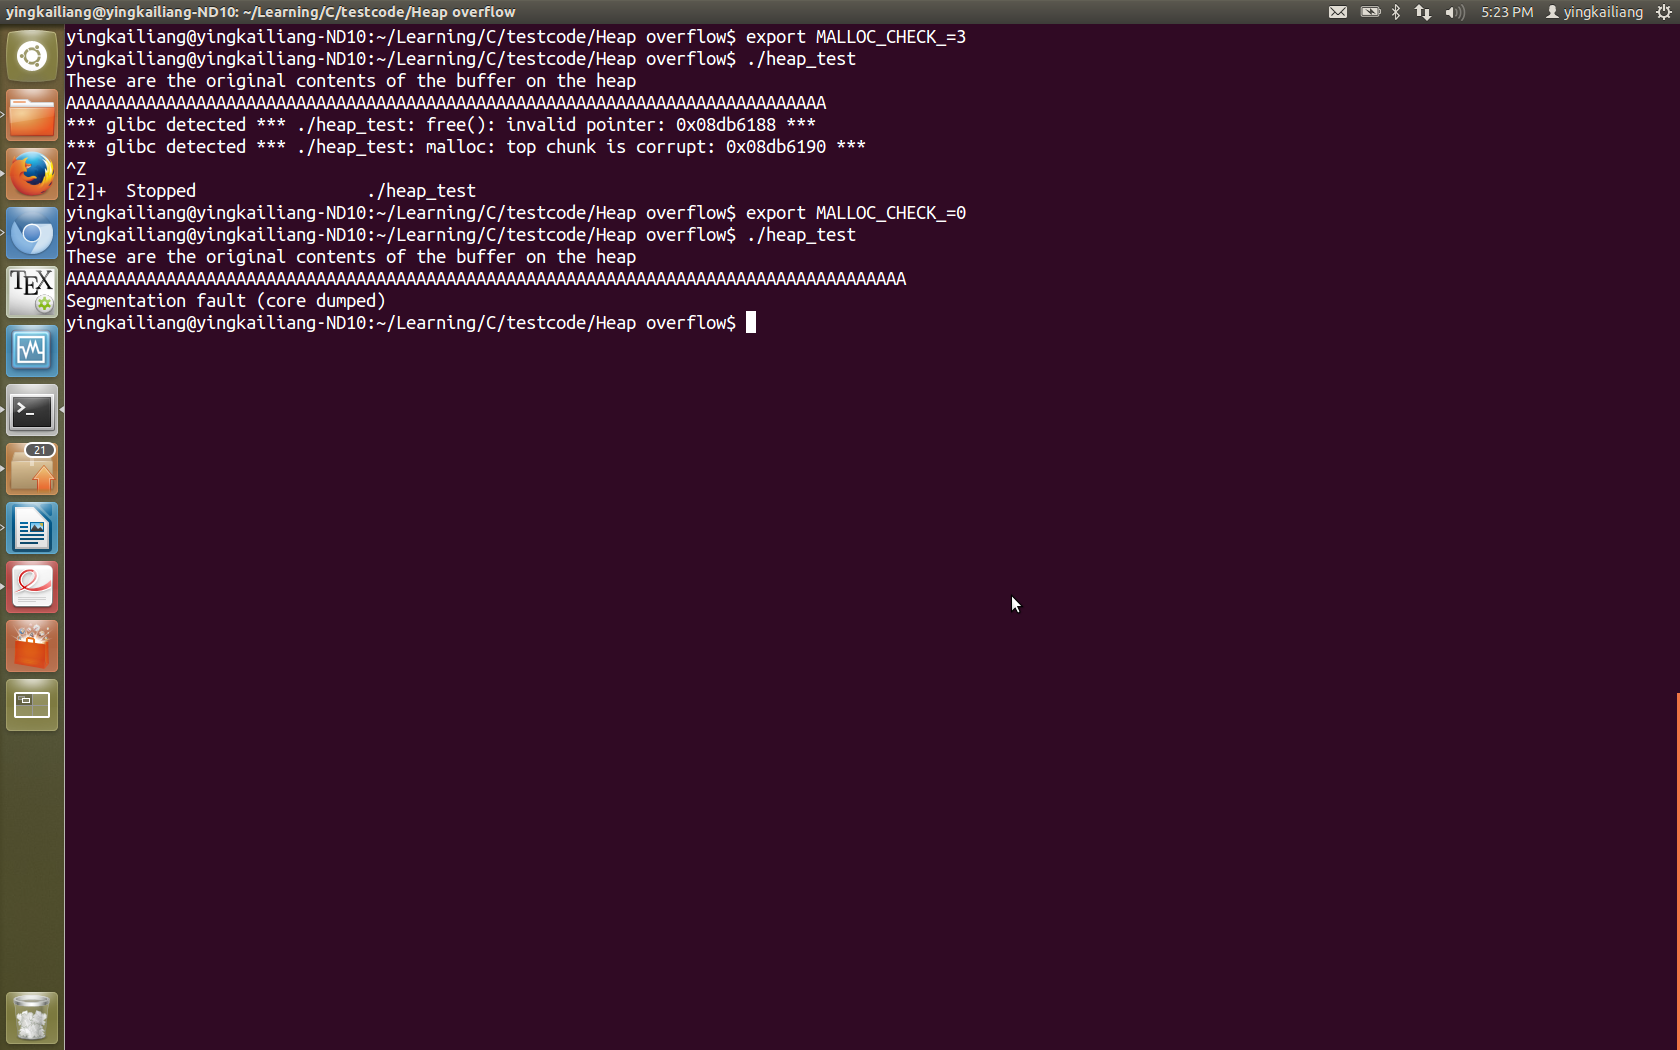
\includegraphics[scale=0.3]{Malloc_check.png}

\subsection{vulnerable program}
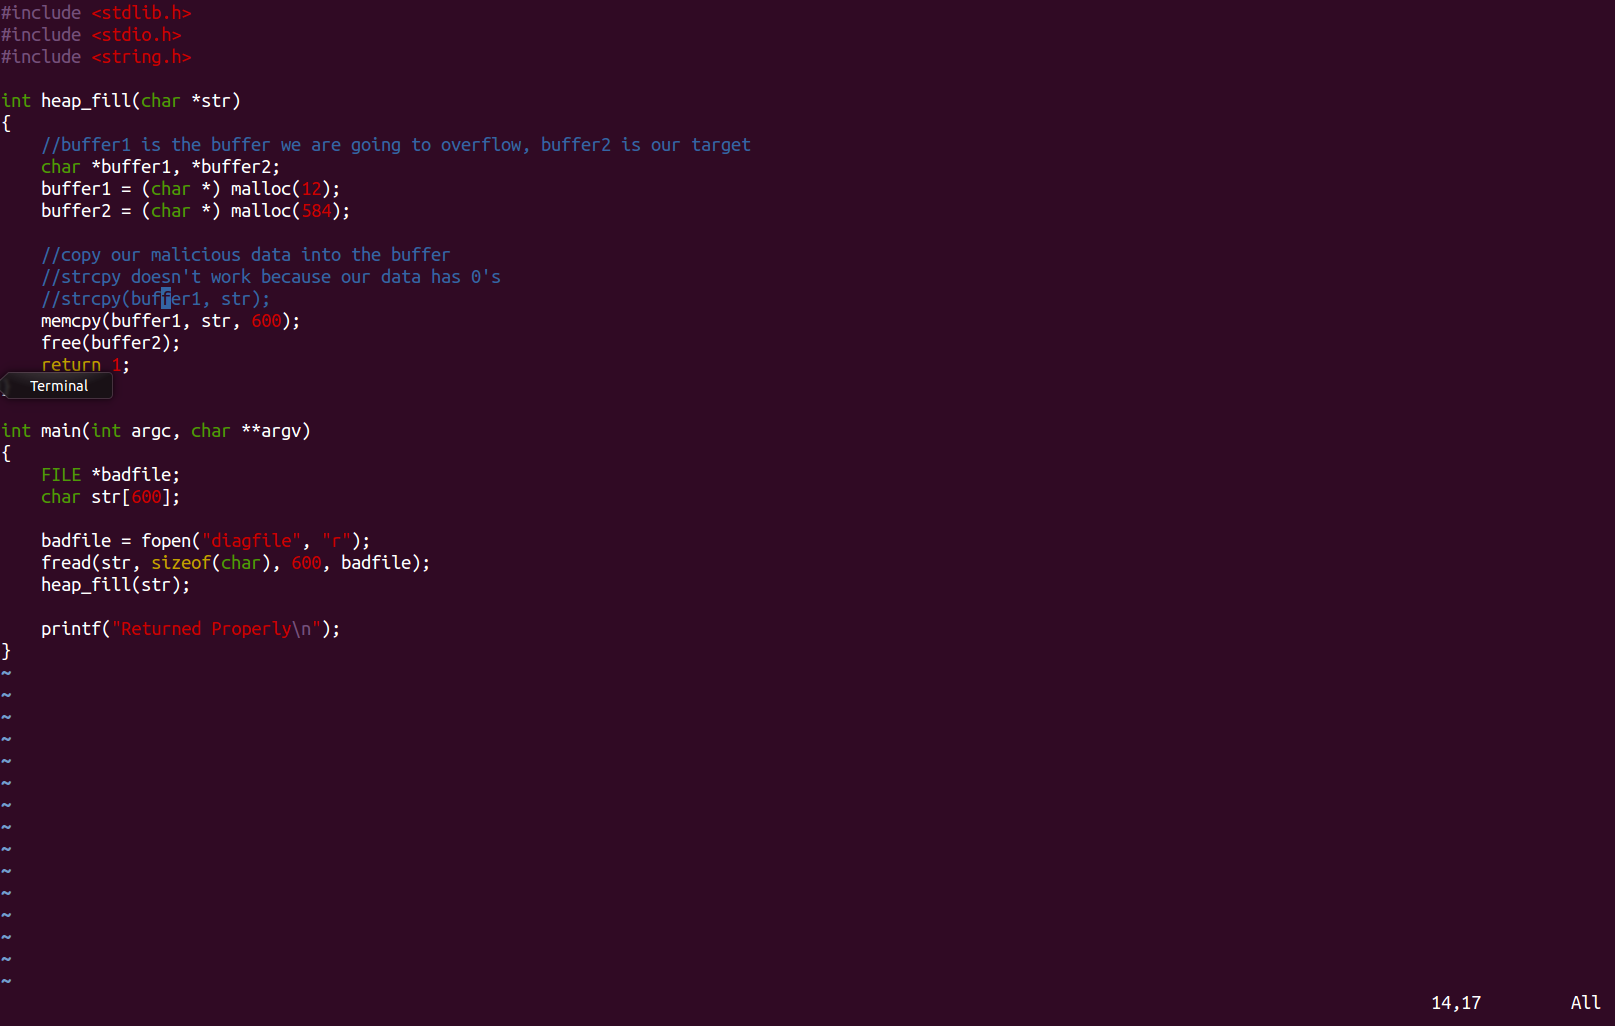
\includegraphics[scale=0.3]{vul_pro.png}

\subsection{hypothetical attack}
Create a fake free chunk,after the chunk we which we need to free. I have fully control of what "fake free chunk" look at. 

The idea is based on glibc malloc.c source code free() function. \\
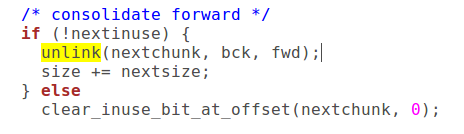
\includegraphics[scale=0.3]{unlink_next_free_chunk.png}
 
How to create this fake chunk:\\

\end{document}
